\chapter{Resultados}

\label{CapResultados}

\section{Precisão do potenciômetro}
A figura \ref{fig:result-resolution} ilustra o ambiente de testes montado para os
testes de resolução do potenciômetro escolhido. Os dados do potenciômetros eram 
enviados a uma placa de prototipagem que implementa uma versão do circuito
de sensoriamento proposto. Para o teste, os dados do arduino foram lidos de 
maneira bruta, o que para um ADC de 10 bits corresponde a valores entre 0 e 1024.

\begin{figure}[h]
    \caption{Ambiente de testes para medida de resolução do sensor.}

    \begin{centering}
        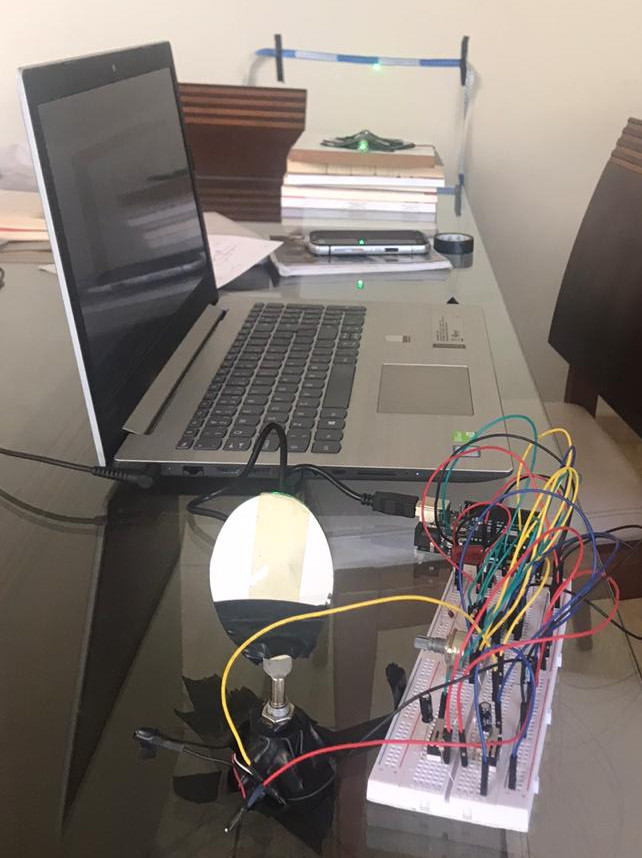
\includegraphics[width=0.5\columnwidth]{images/resultados/resolution.jpg} 
    \par\end{centering}

    \label{fig:result-resolution}
\end{figure}

O espelho atrelado ao potenciômetro foi então rotacionado manualmente até
que fosse vista uma mudança na leitura pelo Arduino. A distância percorrida
pelo \textit{laser} foi então mensurada com o auxílio de uma fita métrica.

A distância percorrida para esta variação mínima encontrada foi de aproximadamente
3cm, e com uma distância entre o sensor e a parede, mensurada com uma treta,
de aproximadamente 215cm. Com estes valores de $d$ e $D$, foi verificado que a angulação 
capaz de ser detectada pelo sensor foi próximo a 0,4\textdegree, segundo a 
equação \ref{eq:teste-pot}.

Embora o ambiente e os equipamentos de medição utilizados não fossem os mais adequados
para medições precisas, o teste demonstrou que o sensor possui uma resolução próxima 
ao esperado, capaz de fornecer boas informações sobre o posicionamento das juntas.

\section{Circuitos de sensoriamento}

Foi preparado um protótipo da placa de sensoriamento, com dispositivos o mais próximo possível 
dos dispositivos reais projetados. O protótipo montado simulava o funcionamento de uma 
placa, contando com dois sensores do tipo fim-de-curso e uma conexão para um potênciometro.
Os dados dos sensores foram conectados a um CI amplificador que contava com 4 amplificadores
operacionais no mesmo dispositivo, o LM324. Os ganhos dos fim-de-curso foram configurados como 
unitários, de acordo com o esquemático da figura \ref{fig:Esquematico-sensor-switch}, já o ganho
do potenciômetro foi configurado como ajustável a partir de outro potenciômetro, este comum e de
volta única.

As conexões foram feitas completamente através de \textit{jumpers}, assim como pode ser visto na
figura \ref{fig:proto-sensor}.

\begin{figure}[h]
    \caption{Circuito de prototipagem do sensoriamento.}

    \begin{centering}
        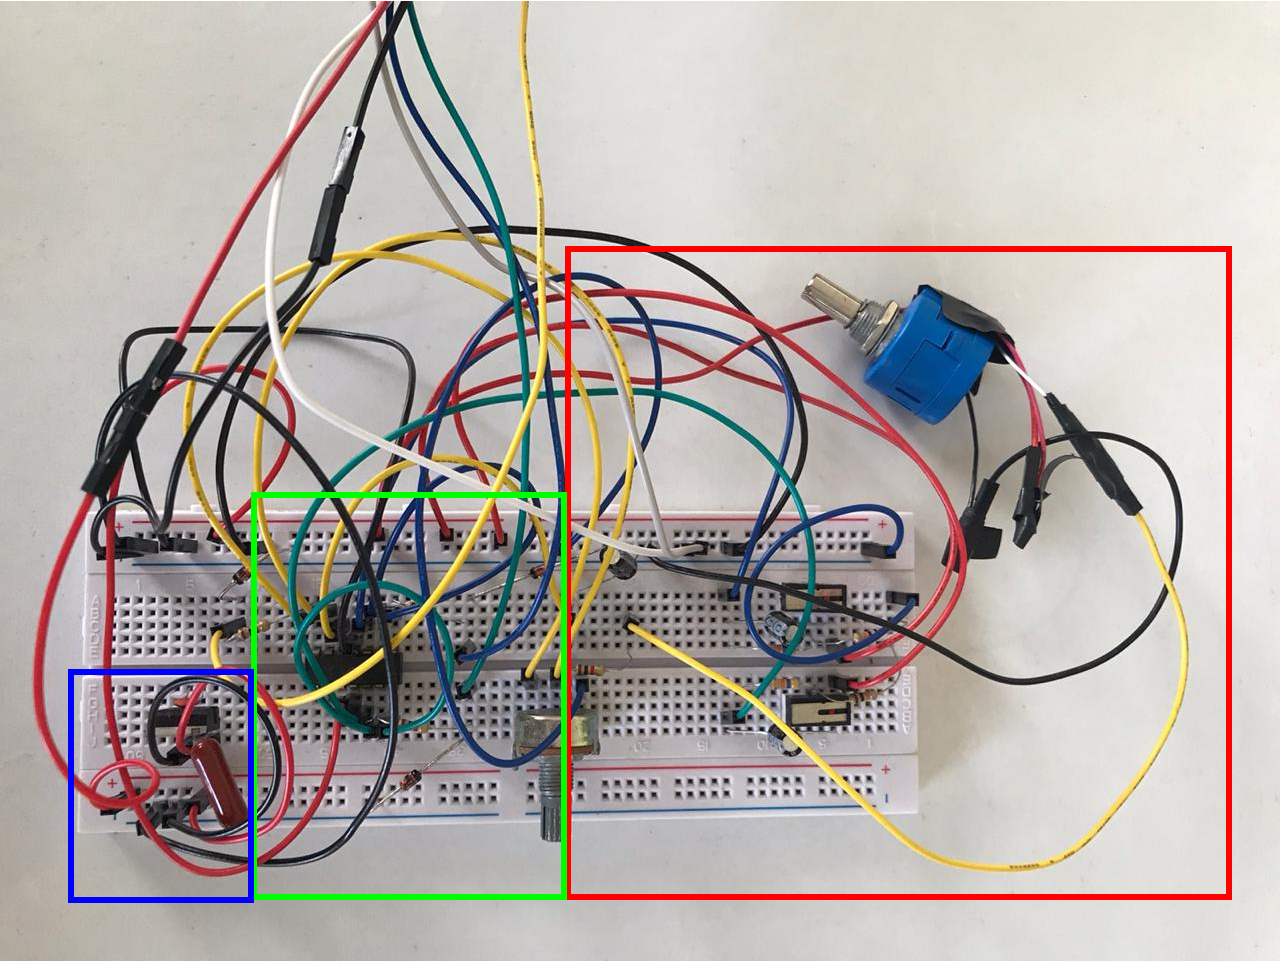
\includegraphics[width=0.75\columnwidth]{images/resultados/proto-sensor.jpeg} 
    \par\end{centering}

    \label{fig:proto-sensor}
\end{figure}

Na figura \ref{fig:proto-sensor} pode ser vista uma divisão espacial dos dispositivos
na placa de prototipagem de acordo com a sua funcionalidade. A área marcada pela
borda na cor vermelha indica os dispositivos sensores e os filtros iniciais de tratamento.
A área verde delimita principalmente a parte dos circuitos ligada a amplificação e à
preparação dos sinais para envio. Por fim, a área azul indica o circuito de alimentação,
com capacitores e regulador de tensão. Os 7 \textit{jumpers} que são vistos saindo da
placa são os que transmitem de fato os sinais para a placa central.

Para os testes e validação destes circuitos, os dados de saída foram conectados
diretamente à placa Arduino. Utilizando programas preparados especificamente para
este teste, foram verificados os valores dos sensores fim-de-curso antes e durante
sua ativação, garantindo que o valor correto seria repassado à etapa posterior
de tratamento. O valor do potenciômetro foi transformado em ângulo através de um
mapeamento linear. 

Foi verificado que para posições do eixo do potenciômetro próximo ao início, 
ocorriam variações indesejadas no valor de leitura, fruto das limitações do sensor.
Para contornar este problema foi definido que o valor mínimo para o qual estas 
variações não ocorrem seria posicionado como valor 0 da junta, limitando o movimento
do atuador para após esta posição por meio do uso dos sensores fim-de-curso.

Os circuitos se comportaram como esperado quando alimentados através de uma fonte de 
12V, com a tensão regulada através do circuito montado.

\section{Jacobiana inversa}

Para validar a sub-rotina que implementa a transformação de velocidades do efetuador final
em velocidades das juntas, foi criado um \textit{script}, assim como já explicado na seção
\ref{sec:analise-cinematica}. A figura \ref{fig:test-vel} ilustra o funcionamento deste teste.

\begin{figure}[ht]
    \caption{Fluxograma programa de validação da jacobiana inversa.}

    \begin{centering}
        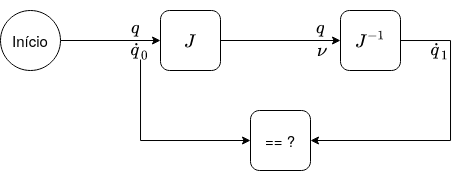
\includegraphics[width=0.6\columnwidth]{images/resultados/Test-vel.png} 
    \par\end{centering}

    \label{fig:test-vel}
\end{figure}

Os valores das posições e velocidades das juntas, $q$ e $\dot{q}$, são definidos no início do programa
e utilizados para calcular a velocidade do efetuador final, tomando-se como caminho de execução uma 
cinemática direta do manipulador. O vetor de velocidades obtido, $\nu$, é então repassado à função
que implementa a inversa da jacobiana, juntamente com o vetor original de posições, para se obter um 
novo vetor de velocidade das juntas, a ser comparado com o vetor original de velocidades.

Foi verificado que para determinados valores das juntas o resultado final obtido era diferente do resultado
inicial configurado. Uma dessas configurações, e o seu valor final obtido, pode ser visto na tabela 
\ref{tab:res-jacobiana}.

\begin{table}[ht]
    \begin{centering}    
    
    \caption{Exemplo de resultado para conversão de velocidade.}
    
    \begin{tabular}{|c|c|c|c|}
        \hline
        $q$ & $\dot{q}_0$ & $\nu$ = $J(q).\dot{q}_0$ & $\dot{q}_1$ = $J^{-1}(q).\nu$ \tabularnewline
        \hline
        \hline
        $\pi/2$ & 0,21 & -0,08 & 0,21  \tabularnewline
        \hline
        $0$ & 0,14 & -0,55 & 0,11 \tabularnewline
        \hline
        $\pi/2$ & 0,85 & 0,04 & -0,11 \tabularnewline
        \hline
        $0$ & 0,01 & 0,88 & 0,88 \tabularnewline
        \hline
        $-\pi/2$ & 0,05 & -0,92 & 0,05  \tabularnewline
        \hline
        $0$ & 0,12 & 0,21 & 0,00 \tabularnewline
        \hline
    \end{tabular}

\label{tab:res-jacobiana}
    
\par\end{centering}
\end{table}

Foi constatado que estas discrepâncias eram resultado de um fator já esperado no uso
da jacobiana inversa, os pontos de singularidade. Com o valor da junta 5 na tabela
\ref{tab:res-jacobiana}, o determinante da equação \ref{eq:det} seria igual a 0, o que 
acarretaria em uma matriz inversa com termos tendendo a $\pm\infty$, ou indeterminações.
Pelo método em que o cálculo da matriz foi organizado, foi possível arranjar alguns termos de 
modo que estas singularidades matemáticas não afetassem todas as juntas, o que é indicado pelo
fato que os termos 1 e 5 apresentaram valores iguais aos originais.
Para demais valores de ângulos, que não resultam em singularidades, os valores obtidos após
a multiplicação por $J^{-1}$ foram iguais ao valores iniciais.

A tentativa de otimizar os cálculos da matriz inversa, evitando o processamento gerado
por um código com diversos laços de repetição, resultou em uma função linear com 126
multiplicacões, 51 somas e 27 variáveis auxiliares. Frente a um código simples que calcularia
a inversa em $6^3$ iterações, o resultado obtido se mostrou satisfatório, mesmo quando aplicado
em um sistema embarcado, fornecendo resultados corretos em um bom tempo.

\section{Circuito central}

Em relação ao circuito central, por este ser composto de uma quantidade grande de 
dispositivos, foi idealizado um protótipo que agrupa as funções básicas de leitura
e tratamento dos sinais de uma única placa de sensoriamento e de acionamento de um
único motor de passo e um motor DC. o sistema completo pode ser visto na figura
\ref{fig:proto-main}.

\begin{figure}[ht]
    \caption{Circuito de prototipagem da placa central.}

    \begin{centering}
        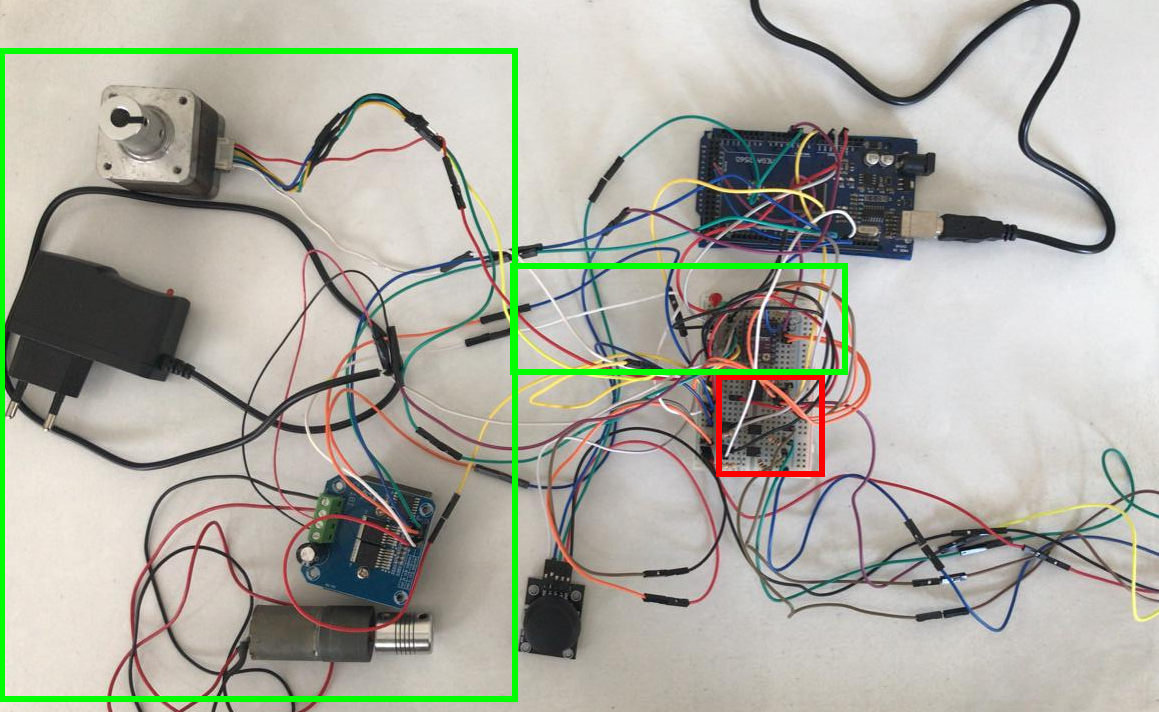
\includegraphics[width=1\columnwidth]{images/resultados/proto-main.jpeg} 
    \par\end{centering}

    \label{fig:proto-main}
\end{figure}

Nas áres indicadas pela cor verde, na figura \ref{fig:proto-main}, são vistos os 
dispositivos \textit{drivers} e seus respectivos atuadores, bem como a fonte de 
alimentação utilizada nos testes para a potência destes.
A área em vermelho indica os dispositivos que realizam o tratamento dos sinais 
provindos da outro placa de prototipagem, como optoacopladores e amplificador operacional.
Na figura podem ser vistos também o \textit{joystick} KY-023 utilizado e um Arduino Mega,
utilizados para interfaceamento com o usuário e processamento geral dos dados, respectivamente.

Nota-se que os atuadores empregados não são de fato iguais aos atuadores escolhidos para o 
sistema. Para os testes e prototipagem preferiu-se utilizar dispositivos genéricos, a fim 
de verificar a funcionalidade do circuito independente do modelo de atuador utilizado.

Foram realizados testes tanto para a simulação do sistema quanto para dados reais resultantes
da ativação dos atuadores, verificando e validando a relação e os diversos circuitos
que compõem o sistema. Como não haviam atuadores de teste suficientes para simular completamente
o circuito, foram realizadas combinações entre leitura real e simulação das juntas.

\section{Controle}

\subsection{Tempo de execução do laço de repetição}

Foi verificado o tempo de execução para cada iteração do laço de repetição principal do
programa de controle, com as funções indicadas no fluxograma \ref{fig:fluxograma}.
Os tempos de execução observados ficaram entre 4 e 5ms, com a inclusão da rotina 
de envio dos dados ao computador, um tempo máximo de 7ms foi observado.

Vale a pena ressaltar que os tempos de execução não estarão sempre entre os valores
observados, sendo possível que alguma iteração do laço apresente maior tempo de 
duração, a depender de interrupções e outros fatores relativos ao sistema. No entanto,
os valores médios observados demonstraram uma boa resposta geral do sistema, com bom
tempo de resposta aos comandos humanos.

\subsection{Simulação}

Para simulação, definiu-se a diretiva ``\textit{SIMULATION}'' como 1 e então o sistema
foi energizado, para dar início ao seu funcionamento. Ao se iniciar a interface
em \textit{python} que se comunica com o circuito, é montada uma representação do 
manipulador utilizando os dados recebidos. A posição inicial foi definida para a simulação
como valores zero para as juntas com motores DC e os valores pós-calibração para as juntas 
com motores de passo. A figura \ref{fig:pos-inicial} ilustra o modelo gerado pelo simulador
assim que a aplicação é iniciada.

\begin{figure}[h]
    \caption{Ambiente de simulação com posição inicial.}

    \begin{centering}
        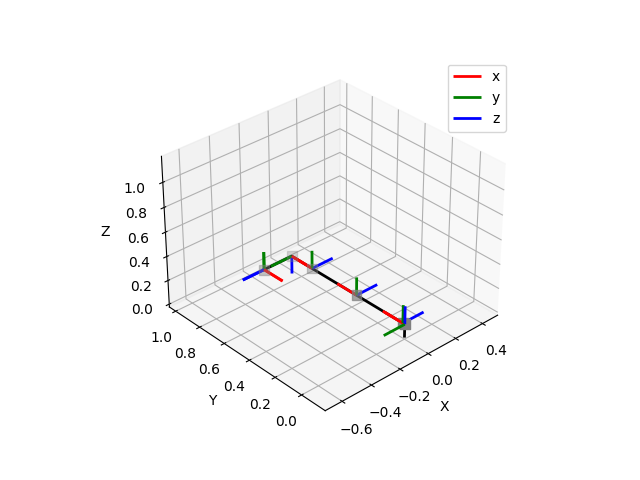
\includegraphics[width=0.8\columnwidth]{images/resultados/pos_inicial.png} 
    \par\end{centering}

    \label{fig:pos-inicial}
\end{figure}

Foi realizada uma tentativa de transportar o braço para a sua configuração zero, 
ou seja, com $\theta_i=0$ para $i$ de 1 a 6, para verificar a controlabilidade do sistema. 
O resultado obtido pode ser visto na figura \ref{fig:pos-zero}.

\begin{figure}[h]
    \caption{Ambiente de simulação com posição zero.}

    \begin{centering}
        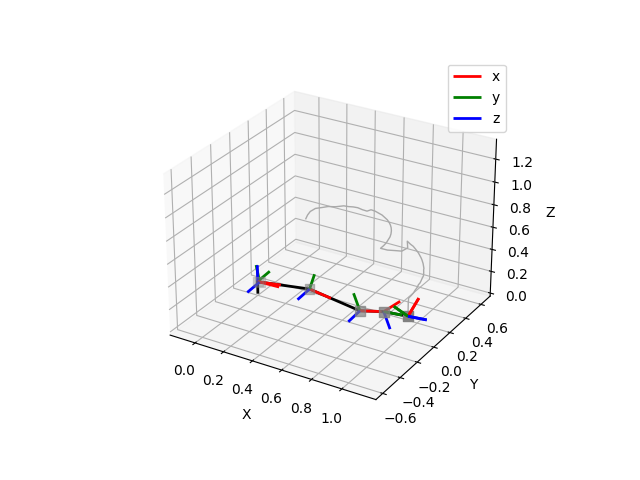
\includegraphics[width=0.8\columnwidth]{images/resultados/pos_zero.png} 
    \par\end{centering}

    \label{fig:pos-zero}
\end{figure}

Esta movimentação poderia ser realizada de vários modos, optou-se por agir sobre o eixo
da junta 5 para deixar o elo seguinte alinhado com o eixo $x$, utilizando o plano $R1$, e em 
seguindo rotacionar o braço em torno da base utilizando o plano $XY$ e informando uma velocidade
desejada na diagonal. Como o plano inicial definido no programa é o plano de translação $XY$,
foi necessário pressionar o botão do \textit{joystick} 2 vezes, alternando para o eixo $R1$ e depois mais
2 vezes, para retornar ao eixo $XY$. Ao final foi necessário modificar o plano de ação para o $XZ$, 
a fim de realizar um ajuste mais fino sobre a altura da posição desejada.

Nota-se na figura \ref{fig:pos-zero} uma indicação do trajeto percorrido pelo ponto final do 
manipulador. Esta trajetória é gerada com base nas velocidades impostas sobre as juntas, que 
se movem de acordo a tentar respeitar a velocidade desejada pelo usuário.

O processo foi repetido tentando atingir outras posições e orientações para o robô, algumas dessas
configurações estão dispostas nas imagens \ref{fig:pos-varias}(a)-(e).

\begin{figure}[h!]
    \begin{centering}

    \begin{floatrow}

        \subfloat[Braço posicionado no alto.]{
            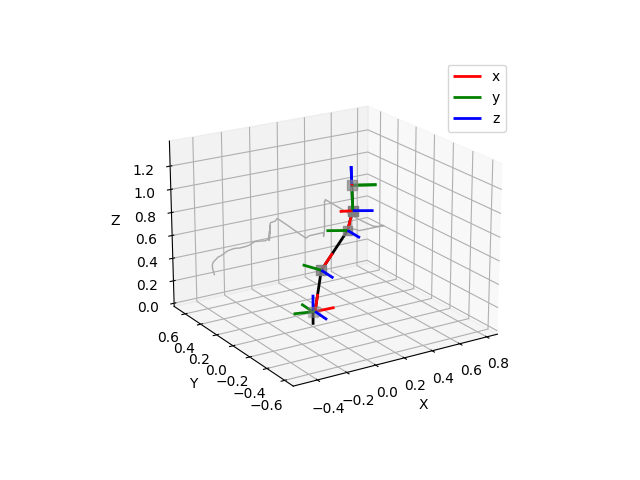
\includegraphics[width=0.5\columnwidth]{images/resultados/pos_z.png}
        }

        \subfloat[Braço na posição de alimentação.]{
            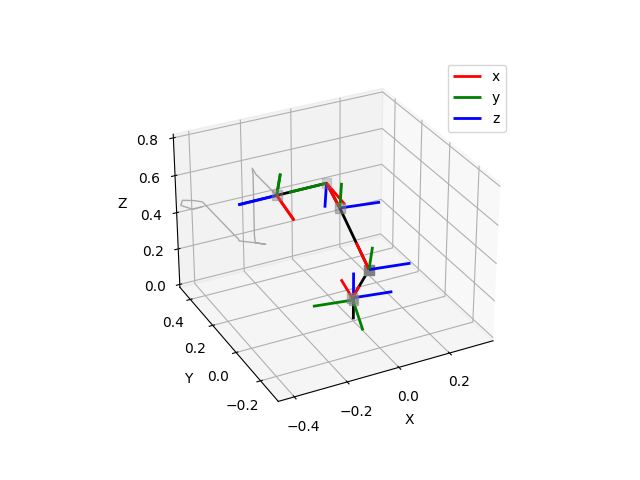
\includegraphics[width=0.5\columnwidth]{images/resultados/pos_alimento.png}
        }

    \end{floatrow}

    \begin{floatrow}

        \subfloat[Braço para pegar objetos na frente do usuário - alto.]{
            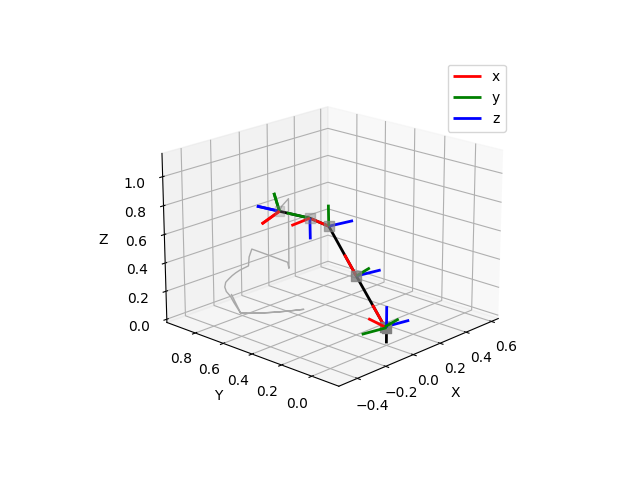
\includegraphics[width=0.5\columnwidth]{images/resultados/pos_pegar1.png}
        }
    
        \subfloat[Braço para pegar objetos na frente do usuário - baixo.]{
            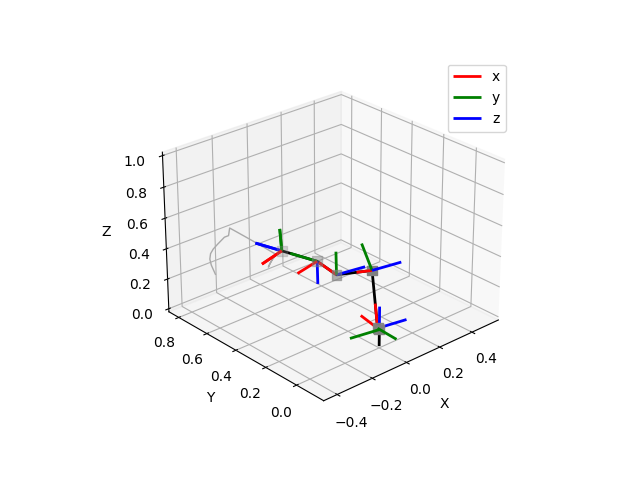
\includegraphics[width=0.5\columnwidth]{images/resultados/pos_pegar2.png}
        }
    
    \end{floatrow}

    \subfloat[Braço na posição de singularidade.]{
        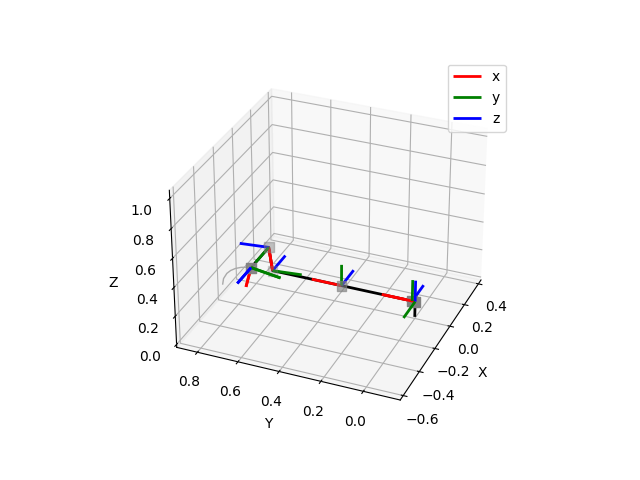
\includegraphics[width=0.5\columnwidth]{images/resultados/pos_singularidade.png}
    }

\caption{Diversas configurações do manipulador simulado.}
\label{fig:pos-varias}

\par\end{centering}
\end{figure}

Alguns pontos de interesse foram os pontos de singularidade do robô. Nestes pontos, é comum
que haja a perda de um dos graus de liberdade do manipulador. A figura \ref{fig:pos-varias}(e) 
ilustra este fato, onde o ângulo de $\theta_5 = -\pi/2$ gera uma singularidade apontada previamente.
Neste ponto específico, os eixos $\hat{Z}_4$ e $\hat{Z}_6$ se tornam coplanares, portanto uma 
rotação em torno de $\hat{Y}_5$ acaba gerando uma indefinição sobre qual dos ângulos deve ser
atuado. Nota-se pelo resultado obtido que a geração de velocidades pela jacobiana favorece a atuação
na junta 4.

\subsection{Atuadores reais}

Para os testes com atuadores reais, foram preparados um motor de passo e um motor DC. Cada
sistema de motor foi marcado de certo modo a permitir a identificação de sua rotação efetiva. 

Inicialmente, ao invés de utilizar dados de simulação, o programa foi modificado para realizar 
a leitura real da junta 1, e a esta junta foi atrelado logicamente um motor de passo, via definição em código. 
Foi realizado então o mesmo procedimento utilizado para geração dos resultados da figura 
\ref{fig:pos-zero}, observando a rotação do motor de passo. Os resultados reais obtidos 
com o atuador para esta junta estão organizados na figura \ref{fig:result-stepper}.
Para indicar que o ponto de calibração foi atingido, foi utilizado um dos sensores da placa 
de prototipagem de sensoriamento.

\begin{figure}[h!]
    \begin{centering}

    \begin{floatrow}

        \subfloat[Motor de passo na posição pós-calibração.]{
            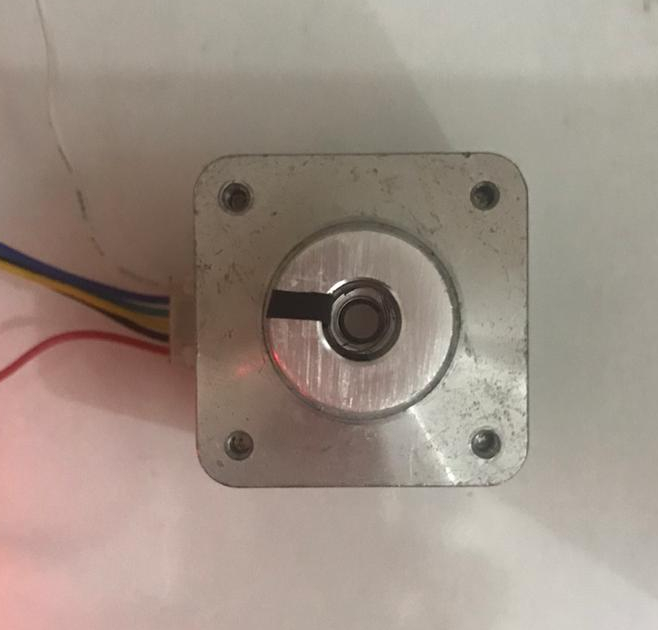
\includegraphics[width=0.3\columnwidth]{images/resultados/stepper1.jpeg}
        }

        \subfloat[Motor de passo após atingir posição desejada.]{
            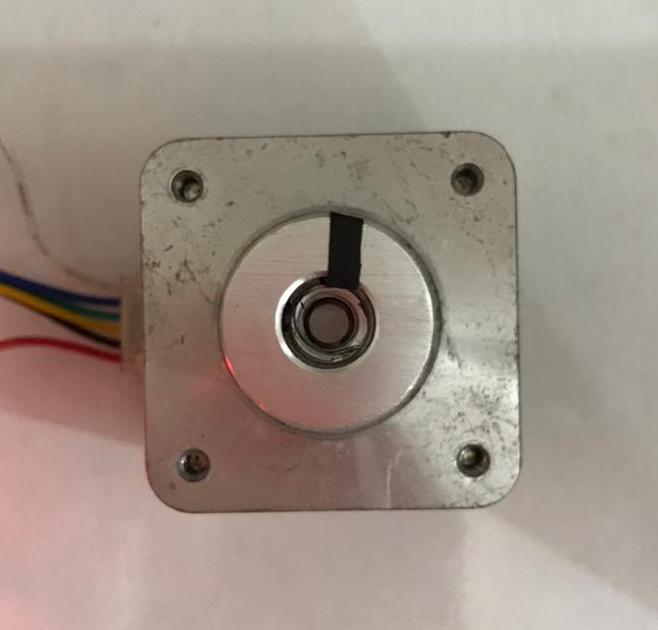
\includegraphics[width=0.3\columnwidth]{images/resultados/stepper2.jpeg}
        }

    \end{floatrow}

    \subfloat[Posição final obtida.]{
        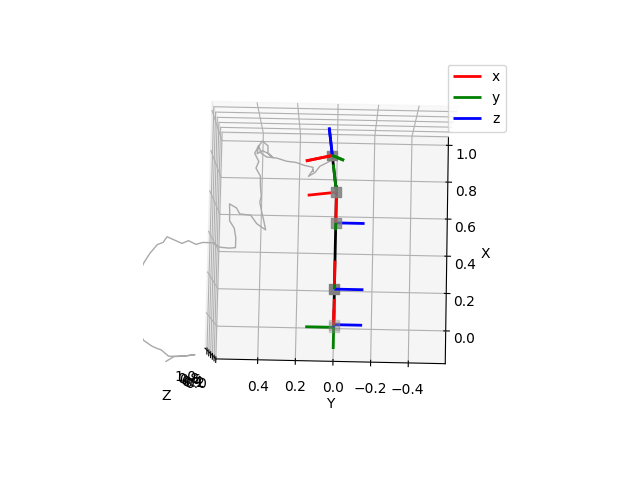
\includegraphics[width=0.8\columnwidth]{images/resultados/pos_stepperfinal.png}
    }

\caption{Resultado com atuação de motor de passo.}
\label{fig:result-stepper}

\par\end{centering}
\end{figure}

As figuras \ref{fig:result-stepper}(a) e \ref{fig:result-stepper}(b) indicam que a rotação
real obtida com os motores de passo aproximou-se da rotação de 90\textdegree\, desejada para
a junta da base. 

Experimentos semelhantes foram realizados para as juntas 5 e 6, que também utilizam motores 
de passo. Os resultados reais de posicionamento foram comparados visualmente com os resultados
obtidos com a animação no ambiente de simulação. Em especial, foram utilizados os planos de ação
$R1$ e $R2$, que permitem atuar diretamente sobre os motores destas juntas, por estarem
relacionados com a rolagem e guinada do punho.
Visualmente, o atuador de teste acompanhou de fato o movimento imposto para o manipulador através das 
velocidades definidas no \textit{joystick}.

Para as outras juntas, que utilizam motores DC, foi preparado um ambiente de testes que consistia
no acoplamento direto entre o eixo de saída de um motor DC de teste e um potenciômetro, assim
como demonstra a figura \ref{fig:teste-dc}. Ambos motor e sensor foram fixados de modo a fornecer
uma resistência contra rotação que não fosse do eixo próprio.

\begin{figure}[h!]
    \begin{centering}

    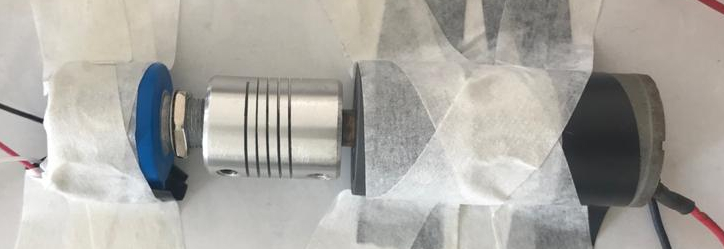
\includegraphics[width=0.8\columnwidth]{images/resultados/teste-dc.jpeg}

\caption{Montagem de teste para motores DC.}
\label{fig:teste-dc}

\par\end{centering}
\end{figure}

A rotina realizada foi semelhante àquela dos motores de passo: Foram conferidas as posições iniciais
indicadas na simulação e no sistema real, e estas foram posteriormente comparadas após uma
sequência de comandos de velocidades informadas via \textit{joystick}. O motor DC foi atribuído à junta 2,
o ombro do sistema. 
A figura \ref{fig:result-dc} agrupa as posições observadas, tanto no ambiente de simulação quanto no ambiente 
real. O ganho do sensor foi ajustado via potenciômetro na placa de prototipagem do sensoriamente para
aproximadamente 2, isto é visível pela figura \ref{fig:result-dc}, onde a simulação indica uma variação
angular próxima a 45\textdegree, mas o sistema real aponta algo mais próximo de 90\textdegree.

\begin{figure}[h!]
    \begin{centering}

    \begin{floatrow}

        \subfloat[Motor DC na posição inicial.]{
            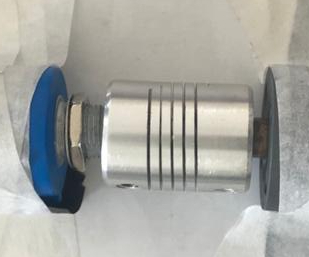
\includegraphics[width=0.4\columnwidth]{images/resultados/dc-real1.jpeg}
        }

        \subfloat[Motor DC na posição final.]{
            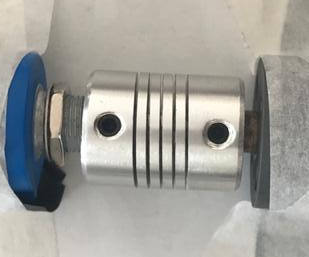
\includegraphics[width=0.4\columnwidth]{images/resultados/dc-real2.jpeg}
        }

    \end{floatrow}

    \begin{floatrow}

        \subfloat[Simulação com valor real de motor DC - inicial.]{
            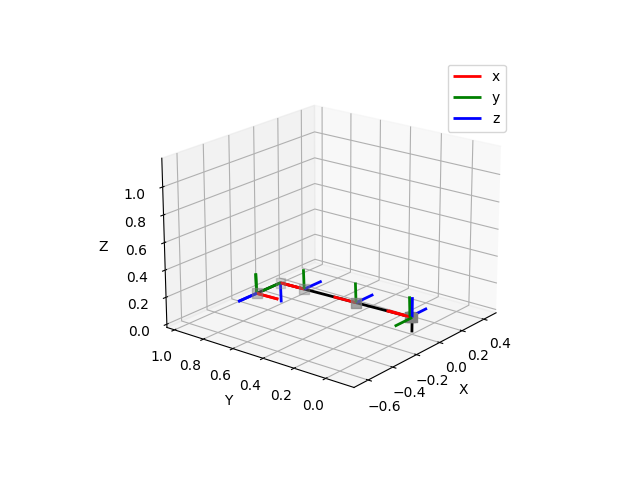
\includegraphics[width=0.5\columnwidth]{images/resultados/pos_dc_inicial.png}
        }

        \subfloat[Simulação com valor real de motor DC - final.]{
            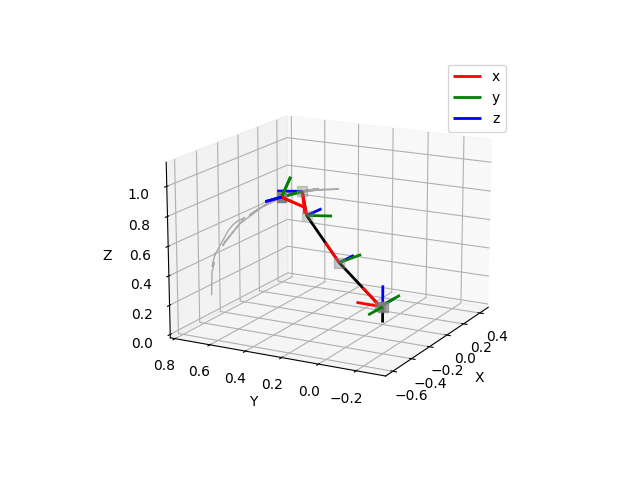
\includegraphics[width=0.5\columnwidth]{images/resultados/pos_dc_final.png}
        }

    \end{floatrow}

\caption{Resultado com atuação de motor de passo.}
\label{fig:result-dc}

\par\end{centering}
\end{figure}

As respostas para ambos os motores foram satisfatórias, indicando a controlabilidade dos 
atuadores via \textit{input} do \textit{joystick} e a correta transmissão dos sinais de leitura. 
Os testes com os sensores potenciômetros de precisão demonstraram que a leitura de posição, 
e consequentemente a resposta de todo o sistema, é favorecida através do uso de toda ou grande
parte da área de trabalho do sensor, utilizando uma transmissão entre o eixo de saída e o eixo
do sensor. 

Os motores DC demonstraram ainda uma dificuldade de trabalho em baixas velocidades, resultando em
complexidades no ajuste fino para o posicionamento final. Acredita-se que este problema será mitigado
no sistema real, pelo uso das relações de transmissão, resultando em uma velocidade mínima menor do que 
a de saída do atuador.

Foi verificado por fim a resposta do sistema com os dados reais dos dois motores, DC e de passo, e complementando
o sistema com a simulação das outras 4 juntas. Uma das posições finais desejadas está disposta na figura 
\ref{fig:pos-dois}, simulando o desejado de obtenção de algum objeto à frente do usuário.

\begin{figure}[h!]
    \begin{centering}

    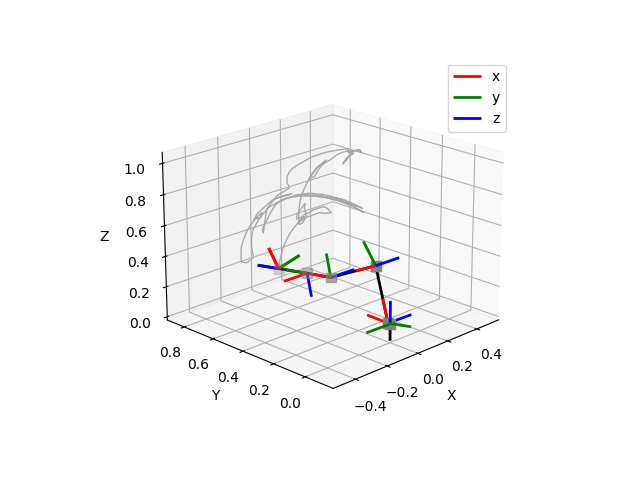
\includegraphics[width=0.8\columnwidth]{images/resultados/pos-dois.png}

\caption{Simulação com dados reais de 2 motores.}
\label{fig:pos-dois}

\par\end{centering}
\end{figure}

A operação do sistema indica o correto funcionamento tanto dos circuitos projetados para atuação e
sensoriamento do braço mecânico. Embora os resultados foram obtidos com protótipos, espera-se que 
os circuitos reais ofereçam resultados similares e/ou melhores, por contarem com dispositivos mais
adequados, seguindo as especificações do projeto.